\documentclass[reprint,unsortedaddress,amsmath,amssymb,floatfix,aps,prl,showkeys]{revtex4-2}
\usepackage{graphicx}% Include figure files
\usepackage{dcolumn}% Align table columns on decimal point
\usepackage{subfigure}
\usepackage{bookmark}
% \usepackage{biblatex}
\usepackage{float}
\usepackage{url}
\usepackage{bm}% bold math
\usepackage{hyperref}% add hypertext capabilities
\usepackage[mathlines]{lineno}% Enable numbering of text and display math

\begin{document}
\title{Memory Matters for Cities}
\author{Gezhi Xiu, Jianying Wang, Lei Dong}
\author{Yu Liu}
\email{liuyu@urban.pku.edu.cn}
\affiliation{Institute of Remote Sensing and Geographic Information System (IRSGIS), Peking University}
\date{\today}

\begin{abstract}
	Empirical evidence suggests that the growth of urban systems is not only determined by local conditions, but also is constrained by regional status. We propose a out-of-equilibrium model of emerging cities within a given region, which explains the spatial transitions of development focus and urban shrinkage phenomenon in developed cities, while analytically keeping the classical results such as Clark's law for urban population density, and Zipf's law for cities' rank size distributions. We show that the classical results are only valid for cities within developing areas, and various urban diseases are inevitable given the limited regional resources. 
\end{abstract}

\maketitle

Urban growth dynamic has always drawn dramatic attention in the past few decades. To systematically consider it needs a suitable physical assumption, e.g., spatial homogeneity with local shifts of population\cite{PhysRevLett.79.523}, dual mechanisms in spatial attaching\cite{PhysRevX.4.011008}, or matching growth for individual\cite{Li2017Simple} to make urban phenomena explainable and predictable. Existing models have succeeded in explaining regional  This problem lies in two parts, population settlement and economic growth, both of which changes spatially over time. Traditional studies of spatial economics have attempted to construct this phenomenon under equilibrium models of regional urban systems\cite{batty1992form}. These models base their idea on agglomeration economies to explain why urban features tend to gather. However, the dynamics of shifts between urban equilibrium (say, poly-centric transitions of cities), is poorly interpreted throughout these models. First, the initial states of urban structure are mostly isotropic, that the present state of cities may be only one possible state of urban equilibrium. Moreover, urban constructions, especially urban sprawling and urban shrinkage, show that cities are out-of equilibrium systems with unsynchronized growth between infrastructure and population distribution. Second, these models mostly address city agglomeration's benefits by the interaction between pairs of individuals. This brings difficulties in understanding the hierarchy and functional divisions that can be seen in nearly all cities. Yet, separating the growth dynamics of infrastructures and population has not yet been taken serious attention in existing models, though some work in complex networks has realized that preferential attachment has hysteresis effect in building contacts. Lastly, throughout the abundant data describing cities, existing models cannot make quantitative predictions with the more information added. We present in this Letter a stochastic growing model of urban systems, which relies on the assumption that the agglomeration effects of infrastructures and population are separated, which can cause the urban core to shift over time. 

%% 2019-12-18 添加,增加一段讨论城市收缩。

Following the discrimination of growing preferences of population and infrastructures, we omit certain details and focus on the basic growth process over longer period of time. To be precise, we consider that the urban dynamics exhibits strong spatial auto-correlations, that a city share the limited part of regional resources. We thereby build a minimal version of model that replicates the basic properties of urban systems and is able to account for the unforeseen cases both qualitatively and quantitatively. The model we propose is thus the essence of  city mass evolution and regional vicissitude. We focus on newly joint population's attracting the force of infrastructure building, its impact on urban shrinkage in space and regional rank injection. 

We first consider the process of urbanization on individual level. People either form new cities, or join the existing cities. We assume that each of these process happens at a constant rate, that is, the times of forming new cities per unit time is proportional to the existing cities, and the population of newly joint citizen of each cities is proportional to the cities' population. We denote the two proportions as $\beta_1$ and $\beta_2$. These settings are parallel to U. Yule's original model\cite{yule1925ii} based on the observation of older genus and species tend to have existed longer. These setting leads to an exponential waiting time for a city or a citizen attracts a kin to the system. This observation also stands for urban systems under stable socio-economic conditions. % This model can reformulate Zipf's law of rank size distribution of cities, as long as $\beta_1$ approximates $\beta_2$.

In dealing with spatial transition of urban structures, we set up the locating rules for urban population. Assuming that the considered area is in $L\times L$ continuous space with grids (representing urban blocks), corresponding to possessiveness: each grid is owned by the city that governs the first citizen who lands on it. Speaking of two parts of growing process, the locating procedures are defined as follows. The city emerges at a randomly chosen, but untaken place (or the city fails to be established). In every emerged city, a newly joint citizen is \emph{introduced} by a existing citizen, so that she is located at a distance of $r$ near the existing one of a random direction $\theta$. We take $r\lesssim 1$ to make sure that new comer is located at or at the neighbor of invader's block. In global perspective, cities growing process is like a diffusion process with some seed points sprinkled on the area as grids are gradually divided into the regime of growing cities. We name this process as \emph{Spatial Yule Process (SYM)}. As we can see, blocks with more nodes have higher probability to introduce new people nearby. Such natural formation of urban systems resembles the population distribution in emergence of many regional systems with adjustable parameters. But regional growth also face difficulties of economical bottlenecks and the need of balancing regional growths. In the meantime, the regional authority can only devote limited amount of total resource in infrastructure construction. These facts imply that we have to add a limit on growing process to reflect the truth. Thus we introduce a mechanism called the \emph{memory kernel}. It can be interpreted by the following statement: New comers needs supply to settle, thus he carries a \emph{coin} to get her settled. However, the total regional resource is limited that the amount of coin is limited, say $N^*$. So from the $N^*+1$ person that settles in a city of this region, she carries a coin as a pre-comer loses hers. Thus when the regional fortune has all been shared, all money is only transferred to the new comers, to allow their essential needs of infrastructures. 

We now discuss the variables $\beta:=\beta_1/\beta_2$ and $r$. The problem of determining the relative speed of city generation is very reminiscent of some problems encountered in gas physics. It is interesting to investigate the number of cities in a given regions of the same population. Some groups tend to form new cities to have sufficient infrastructures and less diversity of urban output ($\beta\gtrsim 1$) and some cities may go otherwise ($\beta\lesssim 1$). This value is actually a reflection of the intensity of regional industry. Speaking of $r$, the metropolis areas over the world have very different densities. In SYM, it determines the sprawl of a city with given population. It can also be taken as the area proportion for a city in the studied region. On the other hand, it is also constraint of regional growth controlling the expected allowance of cities. We take $r=1/2$ as default simulating condition in this Letter.

As for the size of the memory kernel, $N^*$, we realize that it is related to the authority's financial ability to be supportive of more incomer of the region. The competition of resource is neglectable if population is few. As it grows, cities can only supply those who are young and contributory for urban economics. In our framework, we choose the hard kernel with fix-sized memory kernel, so that the economic process can be captured by the partition of coins in different study areas, say, cities or blocks. More coins distributed in a city leads to more attraction to future residents, the case is the same for blocks. Limited resource leads to resource allocation and regional economy, which changes spatially over time. 

In summary, our restricted growth model is defined under three parameters, $\beta$, $r$, and $N^*$. In every exponential time (before the memory kernel is filled), an existing citizen introduces a new individual located from $(r,\theta)$ of her. Meanwhile a new city is introduced by an existing city in another exponential time at somewhere empty. So that the urban system is growing acceleratingly at the first phase, during which every individual owns a coin with her. In the second phase where the memory kernel is full, i.e. the total population of the region is over $N^*$, only those who own coins (summing up to $N^*$) can introduce new comers near to them in the future. Existing ones lose their ability to introduce gradually and almost surely. We denote the population of a city $i$ at timestep $t_n$ as $N_i(t_n)$. The master equations for the first state when the memory kernel is underfull is 
\begin{align}
    P(N_i(t_{n+1}) = N_i(t_{n})+1) &= \delta_{N_i(t_n)}\cdot\frac{k/\beta_1}{k/\beta_1 + n/\beta_2}\notag \\ &+ \frac{n/\beta_2}{k/\beta_1 + n/\beta_2}\frac{N_i(t_{n})}{\sum_i N_i(t_{n})} \notag \\
    P(N_i(t_{n+1}) = N_i(t_{n})) &= \frac{k/\beta_1}{k/\beta_1 + n/\beta_2}\notag \\ + \frac{n/\beta_2}{k/\beta_1 + n/\beta_2}&\cdot (1-\frac{N_i(t_{n})}{\sum_i N_i(t_{n})}),
\end{align}
while the master equations for the second phase goes to\begin{align}
    &P(N_i(t_{n+1}) = N_i(t_{n})+1)=\frac{i}{N^*}\left(1-\frac{i}{N^*-1}\right)\notag\\
    & P(N_i(t_{n+1}) = N_i(t_{n})-1)=\left(1-\frac{i}{N^*}\right) \cdot \frac{i}{N^*-1}\notag\\
    & P(N_i(t_{n+1}) = N_i(t_{n}))=\left(1-\frac{i}{N^*}\right) \cdot\left(1-\frac{i}{N-1}\right) \notag\\ &\hspace{5cm}+ \frac{i}{N}\cdot\frac{i}{N-1}.
\end{align}
And the direct corollary is that $P(N_i(\infty)))$ will converge to $0$ or $1$ almost surely since the memory kernel is fulfilled. 

% Cities are places that concentrate human innovations and productivities. It has been well studied that urban output grows as fast as urban sizes. This results in some interesting results of urban studies on various scales. For inner-city properties, the classical common knowledge is that the population density decay exponentially from core to periphery; As well as cross-city level, the rank size distribution of cities, known as Zipf's law, is the indicator for how much more attractive a bigger city is than smaller cities. These findings are keys to understanding urban formation patterns. In recent years, researchers in urban studies are devoted to reformulate complex cities with simple rules. 

% While our interest lies in hte spatial distribution of population, there are other feathers of urban growth for which parallels with economical development over geographical space can be drawn, for mathematical methods applied. For example, the rank-frequency distribution of urban population\cite{gabaix1999zipf's}, can be explained using a novel form of the Yule process, first introduced to explain the distribution of the number of species

Depending on the relative importance of city sprawl, emergence rate, and economic constraints, the model predicts the existence of three phases, freely growth phase, spatial constraint phase, and economic constraint phase. From now on, we will assume that $N^*$ and $L$ are large enough so that the free growth phase exists for small values of population. In this phase, cities grow desolately, without being controlled by total resource and space. We now describe two of the most important properties of this phase, stately (1) Zipf's law\cite{gabaix1999zipf's} for rank size distribution of cities' population, and (2) Clark's law for mono-centric cities' population density. 

SYM reformulate an important inter-city relationship named the Zipf's law of population sizes\cite{gabaix1999zipf's}, i.e. the populations of cities distribute as a power of ranks, $f_r(r)\sim r^{-(1+\beta)}$. Recall that the number of individuals $Z_t$ in the system at time $t$ has a geometric distribution\cite{durrett1999essentials}, $P(Z_t=n)=e^{-\beta_1t}(1-\exp(- {\beta_1} t))^{n-1}$, and the second assumption that the number of cities will grow exponentially at rate $k/\beta_1$, if we pick a random city, the time since its first appearance will have an exponential distribution of $\beta_1$. Thus the distribution of the population of a random city is 
\begin{align}
	f(n)=\frac{\beta\Gamma(1+\beta)\Gamma(n)}{\Gamma(n+1+\beta)}\approx Cn^{-1-\beta}, \ \text{as } n\rightarrow\infty,
\end{align}
where $\Gamma(\cdot)$ is the gamma function. Since $\beta$ can be anything positive, we can derive different scaling behaviors by switching $\beta$. The experiments have confirmed our analytic results for the first phase in SYM. A simulated validation for this result can be reflected in pic. \ref{fig:rankditribution}. 
\begin{figure}[t]
    \centering
    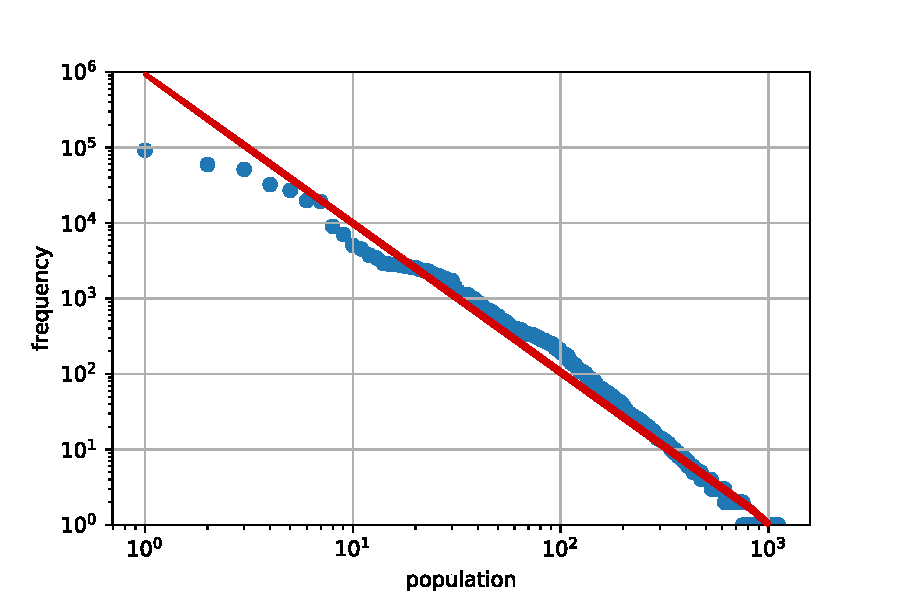
\includegraphics[width=0.48\textwidth]{pics/zipf.pdf}
    \caption{The population distribution as a function of distance from a district's center. The vertical axis is logarithmic processed, which represents the exponential decaying of population distribution. Regardless of the finite-sample effect, we fit the middle part of population density's spatial distribution to the exponential distribution with a slope of $-0.95$, which approximately equals to $1-1/\beta$. This fit has a confidential measurement of $R^2=0.99$.}
    \label{fig:rankditribution}
\end{figure}


% }

% \subfigure[]{
%     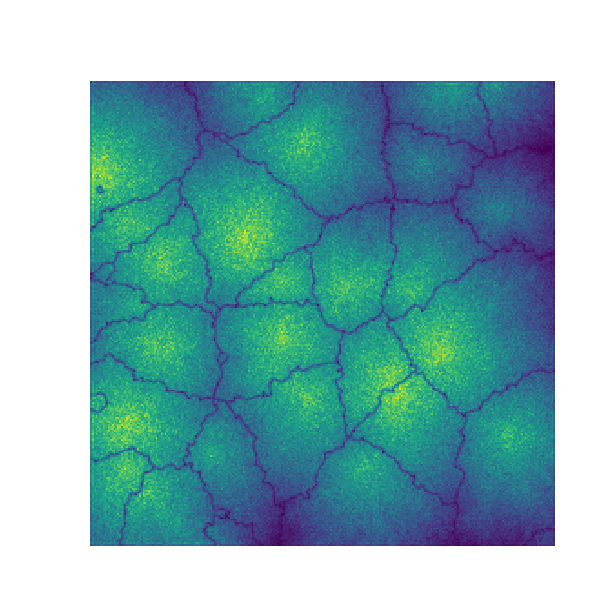
\includegraphics[width=0.3\textwidth]{pics/fractal_41_256.pdf}
%     \label{fig:fractal}
% }

% Adding these facts about area and population distributions, we confirmed the power law scaling behavior between them. This result confirms that the occurrence of universal scaling can be resulted by homogeneous local growth. Noticeably, this result only copes with the case when the space is sufficiently large, so that the population with spatial competition (edging block residents) is small. Simulation confirms our prediction as the slope of log-log plot turns to a flatter phase when population is too large. This can be interpret as the congestion effect, since the competition among cities affects more on larger cities as they control longer boundaries.

%% clark

Inner-city density evolves as a two-dimensional diffusion process, where we can concentrate the density growth dynamics on each axis from the oldest ball of the city. Denote $\rho(d)$ as ball density of sites with the distance $d$ from urban center, and $t_n$ as the time for the $n_{th}$ ball to generate, we have \begin{align}\rho_{t_{n+1}}(d) = (\rho_{t_{n}}(d-r) + \rho_{t_{n}}(d+r) )/2.\label{loc_den}\end{align} By re-scaling time as $\tau_n = t_n\cdot (k\beta_1+N\beta_2)/T$, for a sufficient large $T$, this equation \ref{loc_den} results in a exponential decay of density
    \begin{align}
        \rho(d)\sim e^{-\alpha d}\label{clark_eq}.
    \end{align}
This is a reinvention of \emph{the Clark's} law in empirical urban studies\cite{clark1951urban}. Beyond solitary growth, we analyze the competitiveness of land for different cities. The population within an edging block of city $j$ is estimated by $e^{(T-T_j)}\int_{d}^{d+1}\rho(r)dr/(2\pi d)$, where $T_j$ is the emerging time of city $j$. We also have the waiting time $T_{n+1}-T_{n}\sim 1/n$, and the total population approximation $e^{\beta_1+\beta_2}$, combining which we derive the population of edging blocks if time and the urban radius are given. Since the attractiveness of large urban center is larger, the edging population of large cities is actually smaller than minor cities. We validate our prediction with simulations in \ref{fig:clark} %We give a detailed derivation in Appendix B\ref{edge_comp}.

\begin{figure}
    \centering
    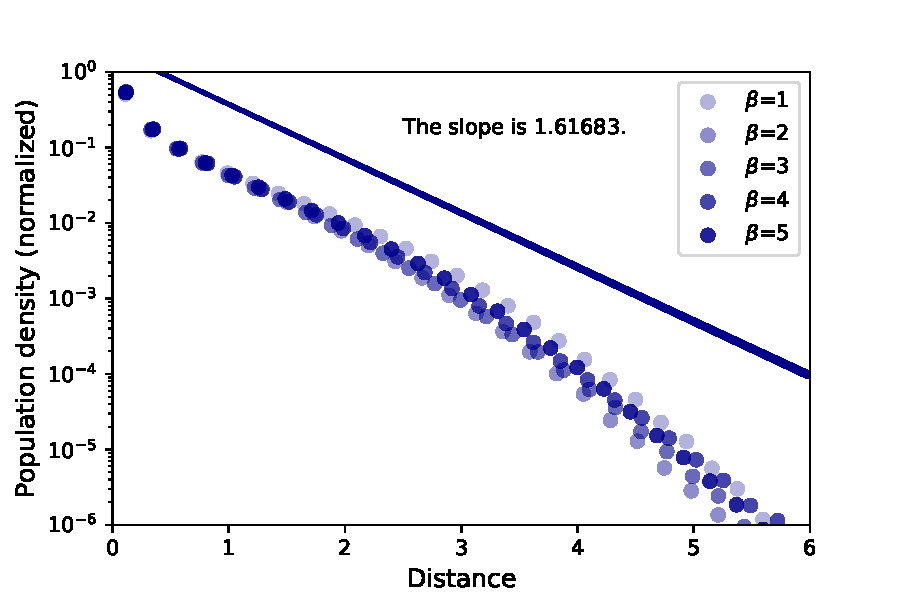
\includegraphics[width=0.48\textwidth]{pics/kernal_density.pdf}
    \caption{The distribution of population among communities. In the simulation we take $N = 10^5$, $\beta_2=1$ and $\beta_1 = 2$. The theoretical prediction of the slope is $-1.5$, and is well approximated by the simulation results.}
    \label{fig:clark}
\end{figure}

%% mk
The multi-dimensional coincidence between the exponents derived in our model and the universal exponents in empirical data of population distribution indicates that only two observation scales lead to the global behaviors of regional growth. Meaning that the urban growth has not yet reached the constrained cases but preventive measures are still necessary.Thus we bring a general constraining parameters $N^*$ to further discuss the second phase of SYM, the resource constrained phase, i.e. the total population reaches $N^*$, the size of memory kernel. Such setting is the abstract of many real-life rules set by global organizations such as the allowance of carbon emissions or sustainable development projects. Each city $i$ has a proportion of population that are labeled as \emph{memorized}, adding up to $\sum_{i=1} m_i(t) = N^*$ for all sufficiently large $t$. If in some period of time, the minor cities generate more offspring than major ones and the superiority of remaining population within the memory kernel changes, minor city will increase its ranking, as the growing rate for each city $i$ is actually $m_i\beta_2$. We now investigate the dynamics within the memory kernel. For each city, $m_i$ acts as a random walk with absorption wall $0$, since no offspring will be expected if no balls are left in the kernel. This result also works for single block case within a city. Denote the population with a block $j$ of city $i$ as $m_{ij}$. According to \cite{durrett1999essentials}, we use a result for branching process that a block loses its vitality if the population goes downhill under a threshold \begin{align}\rho_{threshold} = k\beta_1/(2\beta_2)+N^*/2\end{align}. This value shall be regarded as the sign for urban shrinkage, for the edging blocks have lower density according to equation\ref{clark_eq} thus have a exponentially higher probability to be languished. In other words, urban shrinking shall be reasoned by limited systematic resources.

The last property we come across in SYM is the fractality of urban envelop. Inspired by the multi-player case in fractal financial market, we suppose that the competition at city edges leads to a fractal urban boundary. In SYM, the uncertainty of competition for space lies in $r$. A larger $r$ has larger randomness and brings an extra advantage for minor cities, resulting in a larger fractal dimension. We apply the box counting technique to calculate the fractal dimension of urban envelops, and receive an stable output of $d_f = 1.2\pm 0.05$ with $r = 0.5$, similar to empirical results\cite{batty1992form}. We also find larger $d_f$'s for greater $r$. These results validate our hypothesis that fractal edges coexist with spatial competition. 

%% Discussion

This \emph{letter} concludes the urban system dynamics with only three key components, and receives fruitful results, not only in explaining existing properties, but also predicts . We analytical derive the inter- and intra-city properties Zipf's law of global population, the Clark's law for urban density, and the fractal behaviors of urban edges. Due to the simplicity of SYM, we investigate the future phase transition of urban development in great detail. The results in this paper are derived two assumptions: i) the stationary growing habits as parameters are all set to be constant and ii) the limited resource can be equally treated as a memory kernel. In real life, these assumptions are well-held if the divergence of meta-population across the world is considered. In other words, the identification of a town is 30,000 in Japan, and 200 in Sweden, leading to different considerations of meta-population.Simulations of this model can be adjust to heterogeneous geographical circumstances by applying the growing rate on each block to the product of inherent dynamic $m_{ij}\beta_2$ and the local characteristic $c_{ij}$. The parameter $r$ best determines the type of metropolis over the world for identifying morphology of major cities. Central European cities share lower $r$, making the cities disjoint and centralized; while São Paulo metropolitan area indicates a larger individual preference for urban expansion. Although our results are not all analytically proved, we believe it is a essential step to strip out the power of urban dynamics. The model given in this \emph{letter} is non-commuting, but the community structure is naturally embedded. For further consideration, we can extend the model by adding links as the volume of exploration and preferential return between cities\cite{WANG2019121921}.

The memory kernel mechanism leads to a straightforward corollary that the construction of infrastructure is temporarily ahead of population, as only the people recorded in the kernel are considered as productive people who attract new-comers in the future. This result provides a bottom-up explanation of transition of urban centers. It also tells that the economic growth is a determining factor of human society. Under the circumstances of preferential attraction, if the size of the memory kernel cannot grow fast enough to match with population, the concentration of production will go far from tolerance.

\bibliography{refs.bib}
\end{document}
